\documentclass[twoside]{book}

% Packages required by doxygen
\usepackage{fixltx2e}
\usepackage{calc}
\usepackage{doxygen}
\usepackage{graphicx}
\usepackage[utf8]{inputenc}
\usepackage{makeidx}
\usepackage{multicol}
\usepackage{multirow}
\PassOptionsToPackage{warn}{textcomp}
\usepackage{textcomp}
\usepackage[nointegrals]{wasysym}
\usepackage[table]{xcolor}

% Font selection
\usepackage[T1]{fontenc}
\usepackage{mathptmx}
\usepackage[scaled=.90]{helvet}
\usepackage{courier}
\usepackage{amssymb}
\usepackage{sectsty}
\renewcommand{\familydefault}{\sfdefault}
\allsectionsfont{%
  \fontseries{bc}\selectfont%
  \color{darkgray}%
}
\renewcommand{\DoxyLabelFont}{%
  \fontseries{bc}\selectfont%
  \color{darkgray}%
}
\newcommand{\+}{\discretionary{\mbox{\scriptsize$\hookleftarrow$}}{}{}}

% Page & text layout
\usepackage{geometry}
\geometry{%
  a4paper,%
  top=2.5cm,%
  bottom=2.5cm,%
  left=2.5cm,%
  right=2.5cm%
}
\tolerance=750
\hfuzz=15pt
\hbadness=750
\setlength{\emergencystretch}{15pt}
\setlength{\parindent}{0cm}
\setlength{\parskip}{0.2cm}
\makeatletter
\renewcommand{\paragraph}{%
  \@startsection{paragraph}{4}{0ex}{-1.0ex}{1.0ex}{%
    \normalfont\normalsize\bfseries\SS@parafont%
  }%
}
\renewcommand{\subparagraph}{%
  \@startsection{subparagraph}{5}{0ex}{-1.0ex}{1.0ex}{%
    \normalfont\normalsize\bfseries\SS@subparafont%
  }%
}
\makeatother

% Headers & footers
\usepackage{fancyhdr}
\pagestyle{fancyplain}
\fancyhead[LE]{\fancyplain{}{\bfseries\thepage}}
\fancyhead[CE]{\fancyplain{}{}}
\fancyhead[RE]{\fancyplain{}{\bfseries\leftmark}}
\fancyhead[LO]{\fancyplain{}{\bfseries\rightmark}}
\fancyhead[CO]{\fancyplain{}{}}
\fancyhead[RO]{\fancyplain{}{\bfseries\thepage}}
\fancyfoot[LE]{\fancyplain{}{}}
\fancyfoot[CE]{\fancyplain{}{}}
\fancyfoot[RE]{\fancyplain{}{\bfseries\scriptsize Generated on Sun Dec 7 2014 19\+:36\+:58 for Go Fish by Doxygen }}
\fancyfoot[LO]{\fancyplain{}{\bfseries\scriptsize Generated on Sun Dec 7 2014 19\+:36\+:58 for Go Fish by Doxygen }}
\fancyfoot[CO]{\fancyplain{}{}}
\fancyfoot[RO]{\fancyplain{}{}}
\renewcommand{\footrulewidth}{0.4pt}
\renewcommand{\chaptermark}[1]{%
  \markboth{#1}{}%
}
\renewcommand{\sectionmark}[1]{%
  \markright{\thesection\ #1}%
}

% Indices & bibliography
\usepackage{natbib}
\usepackage[titles]{tocloft}
\setcounter{tocdepth}{3}
\setcounter{secnumdepth}{5}
\makeindex

% Hyperlinks (required, but should be loaded last)
\usepackage{ifpdf}
\ifpdf
  \usepackage[pdftex,pagebackref=true]{hyperref}
\else
  \usepackage[ps2pdf,pagebackref=true]{hyperref}
\fi
\hypersetup{%
  colorlinks=true,%
  linkcolor=blue,%
  citecolor=blue,%
  unicode%
}

% Custom commands
\newcommand{\clearemptydoublepage}{%
  \newpage{\pagestyle{empty}\cleardoublepage}%
}


%===== C O N T E N T S =====

\begin{document}

% Titlepage & ToC
\hypersetup{pageanchor=false,
             bookmarks=true,
             bookmarksnumbered=true,
             pdfencoding=unicode
            }
\pagenumbering{roman}
\begin{titlepage}
\vspace*{7cm}
\begin{center}%
{\Large Go Fish \\[1ex]\large 1.\+1 }\\
\vspace*{1cm}
{\large Generated by Doxygen 1.8.8}\\
\vspace*{0.5cm}
{\small Sun Dec 7 2014 19:36:58}\\
\end{center}
\end{titlepage}
\clearemptydoublepage
\tableofcontents
\clearemptydoublepage
\pagenumbering{arabic}
\hypersetup{pageanchor=true}

%--- Begin generated contents ---
\chapter{Namespace Index}
\section{Namespace List}
Here is a list of all namespaces with brief descriptions\+:\begin{DoxyCompactList}
\item\contentsline{section}{\hyperlink{namespace_go_fish}{Go\+Fish} }{\pageref{namespace_go_fish}}{}
\end{DoxyCompactList}

\chapter{Hierarchical Index}
\section{Class Hierarchy}
This inheritance list is sorted roughly, but not completely, alphabetically\+:\begin{DoxyCompactList}
\item \contentsline{section}{card}{\pageref{classcard}}{}
\item Form\begin{DoxyCompactList}
\item \contentsline{section}{Go\+Fish\+:\+:Form1}{\pageref{class_go_fish_1_1_form1}}{}
\end{DoxyCompactList}
\item \contentsline{section}{Player}{\pageref{class_player}}{}
\item \contentsline{section}{Tree}{\pageref{class_tree}}{}
\end{DoxyCompactList}

\chapter{Class Index}
\section{Class List}
Here are the classes, structs, unions and interfaces with brief descriptions\+:\begin{DoxyCompactList}
\item\contentsline{section}{\hyperlink{classcard}{card} }{\pageref{classcard}}{}
\item\contentsline{section}{\hyperlink{class_go_fish_1_1_form1}{Go\+Fish\+::\+Form1} }{\pageref{class_go_fish_1_1_form1}}{}
\item\contentsline{section}{\hyperlink{class_player}{Player} }{\pageref{class_player}}{}
\item\contentsline{section}{\hyperlink{class_tree}{Tree} }{\pageref{class_tree}}{}
\end{DoxyCompactList}

\chapter{File Index}
\section{File List}
Here is a list of all files with brief descriptions\+:\begin{DoxyCompactList}
\item\contentsline{section}{C\+:/\+Users/\+Tay/\+Desktop/\+T\+N-\/2460701/\+R\+C\+C/\+C\+I\+S-\/17\+C/\+Go Fish -\/ Nesby, Taylor -\/ Final Project -\/ 48596/\+Go Fish/\+Go Fish/\hyperlink{_assembly_info_8cpp}{Assembly\+Info.\+cpp} }{\pageref{_assembly_info_8cpp}}{}
\item\contentsline{section}{C\+:/\+Users/\+Tay/\+Desktop/\+T\+N-\/2460701/\+R\+C\+C/\+C\+I\+S-\/17\+C/\+Go Fish -\/ Nesby, Taylor -\/ Final Project -\/ 48596/\+Go Fish/\+Go Fish/\hyperlink{card_8h}{card.\+h} }{\pageref{card_8h}}{}
\item\contentsline{section}{C\+:/\+Users/\+Tay/\+Desktop/\+T\+N-\/2460701/\+R\+C\+C/\+C\+I\+S-\/17\+C/\+Go Fish -\/ Nesby, Taylor -\/ Final Project -\/ 48596/\+Go Fish/\+Go Fish/\hyperlink{_form1_8h}{Form1.\+h} }{\pageref{_form1_8h}}{}
\item\contentsline{section}{C\+:/\+Users/\+Tay/\+Desktop/\+T\+N-\/2460701/\+R\+C\+C/\+C\+I\+S-\/17\+C/\+Go Fish -\/ Nesby, Taylor -\/ Final Project -\/ 48596/\+Go Fish/\+Go Fish/\hyperlink{_go_01_fish_8cpp}{Go Fish.\+cpp} }{\pageref{_go_01_fish_8cpp}}{}
\item\contentsline{section}{C\+:/\+Users/\+Tay/\+Desktop/\+T\+N-\/2460701/\+R\+C\+C/\+C\+I\+S-\/17\+C/\+Go Fish -\/ Nesby, Taylor -\/ Final Project -\/ 48596/\+Go Fish/\+Go Fish/\hyperlink{_player_8h}{Player.\+h} }{\pageref{_player_8h}}{}
\item\contentsline{section}{C\+:/\+Users/\+Tay/\+Desktop/\+T\+N-\/2460701/\+R\+C\+C/\+C\+I\+S-\/17\+C/\+Go Fish -\/ Nesby, Taylor -\/ Final Project -\/ 48596/\+Go Fish/\+Go Fish/\hyperlink{resource_8h}{resource.\+h} }{\pageref{resource_8h}}{}
\item\contentsline{section}{C\+:/\+Users/\+Tay/\+Desktop/\+T\+N-\/2460701/\+R\+C\+C/\+C\+I\+S-\/17\+C/\+Go Fish -\/ Nesby, Taylor -\/ Final Project -\/ 48596/\+Go Fish/\+Go Fish/\hyperlink{stdafx_8cpp}{stdafx.\+cpp} }{\pageref{stdafx_8cpp}}{}
\item\contentsline{section}{C\+:/\+Users/\+Tay/\+Desktop/\+T\+N-\/2460701/\+R\+C\+C/\+C\+I\+S-\/17\+C/\+Go Fish -\/ Nesby, Taylor -\/ Final Project -\/ 48596/\+Go Fish/\+Go Fish/\hyperlink{stdafx_8h}{stdafx.\+h} }{\pageref{stdafx_8h}}{}
\item\contentsline{section}{C\+:/\+Users/\+Tay/\+Desktop/\+T\+N-\/2460701/\+R\+C\+C/\+C\+I\+S-\/17\+C/\+Go Fish -\/ Nesby, Taylor -\/ Final Project -\/ 48596/\+Go Fish/\+Go Fish/\hyperlink{_tree_8h}{Tree.\+h} }{\pageref{_tree_8h}}{}
\end{DoxyCompactList}

\chapter{Namespace Documentation}
\hypertarget{namespace_go_fish}{\section{Go\+Fish Namespace Reference}
\label{namespace_go_fish}\index{Go\+Fish@{Go\+Fish}}
}
\subsection*{Classes}
\begin{DoxyCompactItemize}
\item 
class \hyperlink{class_go_fish_1_1_form1}{Form1}
\end{DoxyCompactItemize}
\subsection*{Variables}
\begin{DoxyCompactItemize}
\item 
vector$<$ int $>$ \hyperlink{namespace_go_fish_a0516ae63daeafe7d734fd0e380a5cd24}{set}
\item 
deque$<$ \hyperlink{classcard}{card} $>$ \hyperlink{namespace_go_fish_aac69982a27bedb89f2ec4a108be9e7c1}{pool}
\item 
\hyperlink{class_player}{Player} \hyperlink{namespace_go_fish_a9fdd5a69166f90eee7f9717e376ea9bb}{computer}
\item 
\hyperlink{class_player}{Player} \hyperlink{namespace_go_fish_ad4928743b77010f80388ae5f5495bb1b}{person}
\item 
bool \hyperlink{namespace_go_fish_a5ef343351958e4a4c45cfa2d0aa895b5}{wrong} =true
\item 
bool \hyperlink{namespace_go_fish_a76b216755d7556d9ee96ca7ae0fa620d}{time\+To\+Draw} =false
\item 
bool \hyperlink{namespace_go_fish_a1e5e3f29ab64f86a067ee143e1ca2996}{computer\+Turn} =false
\item 
bool \hyperlink{namespace_go_fish_af285f106abe3d068160690d582c4ec70}{time\+To\+Submit} =false
\item 
int \hyperlink{namespace_go_fish_a678c54ee6f4ee2d5eb6ddc8922c1f38d}{person\+Count} =0
\item 
int \hyperlink{namespace_go_fish_a9e05ca6eb20a4dbd5eedd1ed0540de91}{computer\+Count} =0
\end{DoxyCompactItemize}


\subsection{Variable Documentation}
\hypertarget{namespace_go_fish_a9fdd5a69166f90eee7f9717e376ea9bb}{\index{Go\+Fish@{Go\+Fish}!computer@{computer}}
\index{computer@{computer}!Go\+Fish@{Go\+Fish}}
\subsubsection[{computer}]{\setlength{\rightskip}{0pt plus 5cm}{\bf Player} Go\+Fish\+::computer}}\label{namespace_go_fish_a9fdd5a69166f90eee7f9717e376ea9bb}


Definition at line 35 of file Form1.\+h.

\hypertarget{namespace_go_fish_a9e05ca6eb20a4dbd5eedd1ed0540de91}{\index{Go\+Fish@{Go\+Fish}!computer\+Count@{computer\+Count}}
\index{computer\+Count@{computer\+Count}!Go\+Fish@{Go\+Fish}}
\subsubsection[{computer\+Count}]{\setlength{\rightskip}{0pt plus 5cm}int Go\+Fish\+::computer\+Count =0}}\label{namespace_go_fish_a9e05ca6eb20a4dbd5eedd1ed0540de91}


Definition at line 41 of file Form1.\+h.

\hypertarget{namespace_go_fish_a1e5e3f29ab64f86a067ee143e1ca2996}{\index{Go\+Fish@{Go\+Fish}!computer\+Turn@{computer\+Turn}}
\index{computer\+Turn@{computer\+Turn}!Go\+Fish@{Go\+Fish}}
\subsubsection[{computer\+Turn}]{\setlength{\rightskip}{0pt plus 5cm}bool Go\+Fish\+::computer\+Turn =false}}\label{namespace_go_fish_a1e5e3f29ab64f86a067ee143e1ca2996}


Definition at line 39 of file Form1.\+h.

\hypertarget{namespace_go_fish_ad4928743b77010f80388ae5f5495bb1b}{\index{Go\+Fish@{Go\+Fish}!person@{person}}
\index{person@{person}!Go\+Fish@{Go\+Fish}}
\subsubsection[{person}]{\setlength{\rightskip}{0pt plus 5cm}{\bf Player} Go\+Fish\+::person}}\label{namespace_go_fish_ad4928743b77010f80388ae5f5495bb1b}


Definition at line 36 of file Form1.\+h.

\hypertarget{namespace_go_fish_a678c54ee6f4ee2d5eb6ddc8922c1f38d}{\index{Go\+Fish@{Go\+Fish}!person\+Count@{person\+Count}}
\index{person\+Count@{person\+Count}!Go\+Fish@{Go\+Fish}}
\subsubsection[{person\+Count}]{\setlength{\rightskip}{0pt plus 5cm}int Go\+Fish\+::person\+Count =0}}\label{namespace_go_fish_a678c54ee6f4ee2d5eb6ddc8922c1f38d}


Definition at line 41 of file Form1.\+h.

\hypertarget{namespace_go_fish_aac69982a27bedb89f2ec4a108be9e7c1}{\index{Go\+Fish@{Go\+Fish}!pool@{pool}}
\index{pool@{pool}!Go\+Fish@{Go\+Fish}}
\subsubsection[{pool}]{\setlength{\rightskip}{0pt plus 5cm}deque$<${\bf card}$>$ Go\+Fish\+::pool}}\label{namespace_go_fish_aac69982a27bedb89f2ec4a108be9e7c1}


Definition at line 34 of file Form1.\+h.

\hypertarget{namespace_go_fish_a0516ae63daeafe7d734fd0e380a5cd24}{\index{Go\+Fish@{Go\+Fish}!set@{set}}
\index{set@{set}!Go\+Fish@{Go\+Fish}}
\subsubsection[{set}]{\setlength{\rightskip}{0pt plus 5cm}vector$<$int$>$ Go\+Fish\+::set}}\label{namespace_go_fish_a0516ae63daeafe7d734fd0e380a5cd24}
Summary for \hyperlink{class_go_fish_1_1_form1}{Form1} 

Definition at line 33 of file Form1.\+h.

\hypertarget{namespace_go_fish_a76b216755d7556d9ee96ca7ae0fa620d}{\index{Go\+Fish@{Go\+Fish}!time\+To\+Draw@{time\+To\+Draw}}
\index{time\+To\+Draw@{time\+To\+Draw}!Go\+Fish@{Go\+Fish}}
\subsubsection[{time\+To\+Draw}]{\setlength{\rightskip}{0pt plus 5cm}bool Go\+Fish\+::time\+To\+Draw =false}}\label{namespace_go_fish_a76b216755d7556d9ee96ca7ae0fa620d}


Definition at line 38 of file Form1.\+h.

\hypertarget{namespace_go_fish_af285f106abe3d068160690d582c4ec70}{\index{Go\+Fish@{Go\+Fish}!time\+To\+Submit@{time\+To\+Submit}}
\index{time\+To\+Submit@{time\+To\+Submit}!Go\+Fish@{Go\+Fish}}
\subsubsection[{time\+To\+Submit}]{\setlength{\rightskip}{0pt plus 5cm}bool Go\+Fish\+::time\+To\+Submit =false}}\label{namespace_go_fish_af285f106abe3d068160690d582c4ec70}


Definition at line 40 of file Form1.\+h.

\hypertarget{namespace_go_fish_a5ef343351958e4a4c45cfa2d0aa895b5}{\index{Go\+Fish@{Go\+Fish}!wrong@{wrong}}
\index{wrong@{wrong}!Go\+Fish@{Go\+Fish}}
\subsubsection[{wrong}]{\setlength{\rightskip}{0pt plus 5cm}bool Go\+Fish\+::wrong =true}}\label{namespace_go_fish_a5ef343351958e4a4c45cfa2d0aa895b5}


Definition at line 37 of file Form1.\+h.


\chapter{Class Documentation}
\hypertarget{classcard}{\section{card Class Reference}
\label{classcard}\index{card@{card}}
}


{\ttfamily \#include $<$card.\+h$>$}

\subsection*{Public Member Functions}
\begin{DoxyCompactItemize}
\item 
\hyperlink{classcard_a42e864c677c1f99451d3adf308535922}{card} (string d, int v)
\item 
string \hyperlink{classcard_a3b7b3442aac023d3613b256c05b29eb0}{get\+Desc} ()
\item 
int \hyperlink{classcard_a5cf12898a17ff2eda5469eaf857e286d}{get\+Value} ()
\item 
\hyperlink{classcard_aaccc9279ab6da12c111d4d6f5915f29f}{$\sim$card} (void)
\end{DoxyCompactItemize}
\subsection*{Public Attributes}
\begin{DoxyCompactItemize}
\item 
string \hyperlink{classcard_a19812a4daafbfa06456a048352ea7810}{desc}
\item 
int \hyperlink{classcard_a8c8ecc859e715ee6b55bef5d692f508b}{value}
\end{DoxyCompactItemize}


\subsection{Detailed Description}


Definition at line 2 of file card.\+h.



\subsection{Constructor \& Destructor Documentation}
\hypertarget{classcard_a42e864c677c1f99451d3adf308535922}{\index{card@{card}!card@{card}}
\index{card@{card}!card@{card}}
\subsubsection[{card}]{\setlength{\rightskip}{0pt plus 5cm}card\+::card (
\begin{DoxyParamCaption}
\item[{string}]{d, }
\item[{int}]{v}
\end{DoxyParamCaption}
)\hspace{0.3cm}{\ttfamily [inline]}}}\label{classcard_a42e864c677c1f99451d3adf308535922}


Definition at line 7 of file card.\+h.

\hypertarget{classcard_aaccc9279ab6da12c111d4d6f5915f29f}{\index{card@{card}!````~card@{$\sim$card}}
\index{````~card@{$\sim$card}!card@{card}}
\subsubsection[{$\sim$card}]{\setlength{\rightskip}{0pt plus 5cm}card\+::$\sim$card (
\begin{DoxyParamCaption}
\item[{void}]{}
\end{DoxyParamCaption}
)\hspace{0.3cm}{\ttfamily [inline]}}}\label{classcard_aaccc9279ab6da12c111d4d6f5915f29f}


Definition at line 16 of file card.\+h.



\subsection{Member Function Documentation}
\hypertarget{classcard_a3b7b3442aac023d3613b256c05b29eb0}{\index{card@{card}!get\+Desc@{get\+Desc}}
\index{get\+Desc@{get\+Desc}!card@{card}}
\subsubsection[{get\+Desc}]{\setlength{\rightskip}{0pt plus 5cm}string card\+::get\+Desc (
\begin{DoxyParamCaption}
{}
\end{DoxyParamCaption}
)\hspace{0.3cm}{\ttfamily [inline]}}}\label{classcard_a3b7b3442aac023d3613b256c05b29eb0}


Definition at line 12 of file card.\+h.

\hypertarget{classcard_a5cf12898a17ff2eda5469eaf857e286d}{\index{card@{card}!get\+Value@{get\+Value}}
\index{get\+Value@{get\+Value}!card@{card}}
\subsubsection[{get\+Value}]{\setlength{\rightskip}{0pt plus 5cm}int card\+::get\+Value (
\begin{DoxyParamCaption}
{}
\end{DoxyParamCaption}
)\hspace{0.3cm}{\ttfamily [inline]}}}\label{classcard_a5cf12898a17ff2eda5469eaf857e286d}


Definition at line 14 of file card.\+h.



\subsection{Member Data Documentation}
\hypertarget{classcard_a19812a4daafbfa06456a048352ea7810}{\index{card@{card}!desc@{desc}}
\index{desc@{desc}!card@{card}}
\subsubsection[{desc}]{\setlength{\rightskip}{0pt plus 5cm}string card\+::desc}}\label{classcard_a19812a4daafbfa06456a048352ea7810}


Definition at line 5 of file card.\+h.

\hypertarget{classcard_a8c8ecc859e715ee6b55bef5d692f508b}{\index{card@{card}!value@{value}}
\index{value@{value}!card@{card}}
\subsubsection[{value}]{\setlength{\rightskip}{0pt plus 5cm}int card\+::value}}\label{classcard_a8c8ecc859e715ee6b55bef5d692f508b}


Definition at line 6 of file card.\+h.



The documentation for this class was generated from the following file\+:\begin{DoxyCompactItemize}
\item 
C\+:/\+Users/\+Tay/\+Desktop/\+T\+N-\/2460701/\+R\+C\+C/\+C\+I\+S-\/17\+C/\+Go Fish -\/ Nesby, Taylor -\/ Final Project -\/ 48596/\+Go Fish/\+Go Fish/\hyperlink{card_8h}{card.\+h}\end{DoxyCompactItemize}

\hypertarget{class_go_fish_1_1_form1}{\section{Go\+Fish\+:\+:Form1 Class Reference}
\label{class_go_fish_1_1_form1}\index{Go\+Fish\+::\+Form1@{Go\+Fish\+::\+Form1}}
}


{\ttfamily \#include $<$Form1.\+h$>$}



Inheritance diagram for Go\+Fish\+:\+:Form1\+:\nopagebreak
\begin{figure}[H]
\begin{center}
\leavevmode
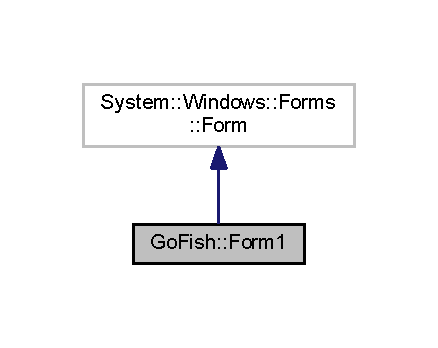
\includegraphics[width=210pt]{class_go_fish_1_1_form1__inherit__graph}
\end{center}
\end{figure}


Collaboration diagram for Go\+Fish\+:\+:Form1\+:\nopagebreak
\begin{figure}[H]
\begin{center}
\leavevmode
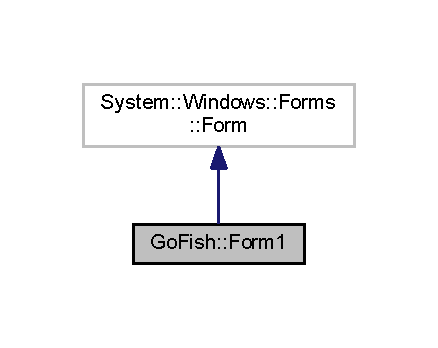
\includegraphics[width=210pt]{class_go_fish_1_1_form1__coll__graph}
\end{center}
\end{figure}
\subsection*{Public Member Functions}
\begin{DoxyCompactItemize}
\item 
\hyperlink{class_go_fish_1_1_form1_a0ce9b0237d4a230cba08fbfa74bb2b02}{Form1} (void)
\item 
System\+::\+Void \hyperlink{class_go_fish_1_1_form1_a31dd106b83b5bf65028eac54f8164368}{start\+Btn\+\_\+\+Click} (System\+::\+Object$^\wedge$sender, System\+::\+Event\+Args$^\wedge$e)
\end{DoxyCompactItemize}
\subsection*{Protected Member Functions}
\begin{DoxyCompactItemize}
\item 
\hyperlink{class_go_fish_1_1_form1_adda5dd1ba5fd7558abe3c0cb2f63611b}{$\sim$\+Form1} ()
\begin{DoxyCompactList}\small\item\em Clean up any resources being used. \end{DoxyCompactList}\end{DoxyCompactItemize}


\subsection{Detailed Description}


Definition at line 43 of file Form1.\+h.



\subsection{Constructor \& Destructor Documentation}
\hypertarget{class_go_fish_1_1_form1_a0ce9b0237d4a230cba08fbfa74bb2b02}{\index{Go\+Fish\+::\+Form1@{Go\+Fish\+::\+Form1}!Form1@{Form1}}
\index{Form1@{Form1}!Go\+Fish\+::\+Form1@{Go\+Fish\+::\+Form1}}
\subsubsection[{Form1}]{\setlength{\rightskip}{0pt plus 5cm}Go\+Fish\+::\+Form1\+::\+Form1 (
\begin{DoxyParamCaption}
\item[{void}]{}
\end{DoxyParamCaption}
)\hspace{0.3cm}{\ttfamily [inline]}}}\label{class_go_fish_1_1_form1_a0ce9b0237d4a230cba08fbfa74bb2b02}


Definition at line 47 of file Form1.\+h.

\hypertarget{class_go_fish_1_1_form1_adda5dd1ba5fd7558abe3c0cb2f63611b}{\index{Go\+Fish\+::\+Form1@{Go\+Fish\+::\+Form1}!````~Form1@{$\sim$\+Form1}}
\index{````~Form1@{$\sim$\+Form1}!Go\+Fish\+::\+Form1@{Go\+Fish\+::\+Form1}}
\subsubsection[{$\sim$\+Form1}]{\setlength{\rightskip}{0pt plus 5cm}Go\+Fish\+::\+Form1\+::$\sim$\+Form1 (
\begin{DoxyParamCaption}
{}
\end{DoxyParamCaption}
)\hspace{0.3cm}{\ttfamily [inline]}, {\ttfamily [protected]}}}\label{class_go_fish_1_1_form1_adda5dd1ba5fd7558abe3c0cb2f63611b}


Clean up any resources being used. 



Definition at line 59 of file Form1.\+h.



\subsection{Member Function Documentation}
\hypertarget{class_go_fish_1_1_form1_a31dd106b83b5bf65028eac54f8164368}{\index{Go\+Fish\+::\+Form1@{Go\+Fish\+::\+Form1}!start\+Btn\+\_\+\+Click@{start\+Btn\+\_\+\+Click}}
\index{start\+Btn\+\_\+\+Click@{start\+Btn\+\_\+\+Click}!Go\+Fish\+::\+Form1@{Go\+Fish\+::\+Form1}}
\subsubsection[{start\+Btn\+\_\+\+Click}]{\setlength{\rightskip}{0pt plus 5cm}System\+::\+Void Go\+Fish\+::\+Form1\+::start\+Btn\+\_\+\+Click (
\begin{DoxyParamCaption}
\item[{System\+::\+Object$^\wedge$}]{sender, }
\item[{System\+::\+Event\+Args$^\wedge$}]{e}
\end{DoxyParamCaption}
)\hspace{0.3cm}{\ttfamily [inline]}}}\label{class_go_fish_1_1_form1_a31dd106b83b5bf65028eac54f8164368}


Definition at line 351 of file Form1.\+h.



Here is the call graph for this function\+:\nopagebreak
\begin{figure}[H]
\begin{center}
\leavevmode
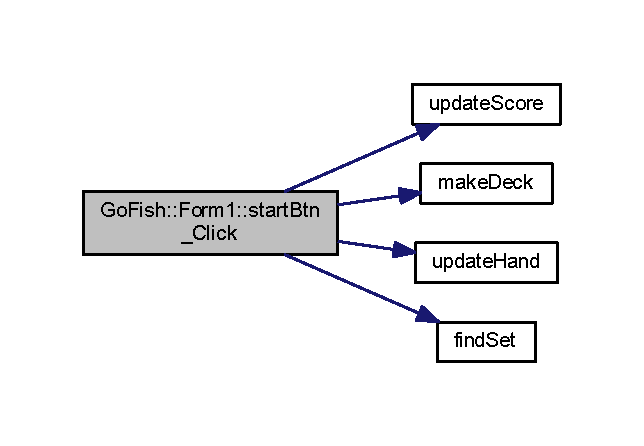
\includegraphics[width=309pt]{class_go_fish_1_1_form1_a31dd106b83b5bf65028eac54f8164368_cgraph}
\end{center}
\end{figure}




The documentation for this class was generated from the following file\+:\begin{DoxyCompactItemize}
\item 
C\+:/\+Users/\+Tay/\+Desktop/\+T\+N-\/2460701/\+R\+C\+C/\+C\+I\+S-\/17\+C/\+Go Fish -\/ Nesby, Taylor -\/ Final Project -\/ 48596/\+Go Fish/\+Go Fish/\hyperlink{_form1_8h}{Form1.\+h}\end{DoxyCompactItemize}

\hypertarget{class_player}{\section{Player Class Reference}
\label{class_player}\index{Player@{Player}}
}


{\ttfamily \#include $<$Player.\+h$>$}

\subsection*{Public Member Functions}
\begin{DoxyCompactItemize}
\item 
\hyperlink{class_player_affe0cc3cb714f6deb4e62f0c0d3f1fd8}{Player} ()
\item 
virtual \hyperlink{class_player_a81b8e12b8f9b1df886bfb5cf4e935f69}{$\sim$\+Player} (void)
\end{DoxyCompactItemize}
\subsection*{Public Attributes}
\begin{DoxyCompactItemize}
\item 
deque$<$ \hyperlink{classcard}{card} $>$ \hyperlink{class_player_afb8208ba11e1635d2c0bb0acd10d0a50}{hand}
\item 
vector$<$ int $>$ \hyperlink{class_player_a259a75b0991b8130c807051225a2e4d5}{guess}
\end{DoxyCompactItemize}


\subsection{Detailed Description}


Definition at line 5 of file Player.\+h.



\subsection{Constructor \& Destructor Documentation}
\hypertarget{class_player_affe0cc3cb714f6deb4e62f0c0d3f1fd8}{\index{Player@{Player}!Player@{Player}}
\index{Player@{Player}!Player@{Player}}
\subsubsection[{Player}]{\setlength{\rightskip}{0pt plus 5cm}Player\+::\+Player (
\begin{DoxyParamCaption}
{}
\end{DoxyParamCaption}
)\hspace{0.3cm}{\ttfamily [inline]}}}\label{class_player_affe0cc3cb714f6deb4e62f0c0d3f1fd8}


Definition at line 12 of file Player.\+h.

\hypertarget{class_player_a81b8e12b8f9b1df886bfb5cf4e935f69}{\index{Player@{Player}!````~Player@{$\sim$\+Player}}
\index{````~Player@{$\sim$\+Player}!Player@{Player}}
\subsubsection[{$\sim$\+Player}]{\setlength{\rightskip}{0pt plus 5cm}virtual Player\+::$\sim$\+Player (
\begin{DoxyParamCaption}
\item[{void}]{}
\end{DoxyParamCaption}
)\hspace{0.3cm}{\ttfamily [inline]}, {\ttfamily [virtual]}}}\label{class_player_a81b8e12b8f9b1df886bfb5cf4e935f69}


Definition at line 14 of file Player.\+h.



\subsection{Member Data Documentation}
\hypertarget{class_player_a259a75b0991b8130c807051225a2e4d5}{\index{Player@{Player}!guess@{guess}}
\index{guess@{guess}!Player@{Player}}
\subsubsection[{guess}]{\setlength{\rightskip}{0pt plus 5cm}vector$<$int$>$ Player\+::guess}}\label{class_player_a259a75b0991b8130c807051225a2e4d5}


Definition at line 11 of file Player.\+h.

\hypertarget{class_player_afb8208ba11e1635d2c0bb0acd10d0a50}{\index{Player@{Player}!hand@{hand}}
\index{hand@{hand}!Player@{Player}}
\subsubsection[{hand}]{\setlength{\rightskip}{0pt plus 5cm}deque$<${\bf card}$>$ Player\+::hand}}\label{class_player_afb8208ba11e1635d2c0bb0acd10d0a50}


Definition at line 9 of file Player.\+h.



The documentation for this class was generated from the following file\+:\begin{DoxyCompactItemize}
\item 
C\+:/\+Users/\+Tay/\+Desktop/\+T\+N-\/2460701/\+R\+C\+C/\+C\+I\+S-\/17\+C/\+Go Fish -\/ Nesby, Taylor -\/ Final Project -\/ 48596/\+Go Fish/\+Go Fish/\hyperlink{_player_8h}{Player.\+h}\end{DoxyCompactItemize}

\hypertarget{class_tree}{\section{Tree Class Reference}
\label{class_tree}\index{Tree@{Tree}}
}


{\ttfamily \#include $<$Tree.\+h$>$}

\subsection*{Public Member Functions}
\begin{DoxyCompactItemize}
\item 
\hyperlink{class_tree_ad376a7c639d857312f5de2ef47482f68}{Tree} ()
\item 
\hyperlink{class_tree_abdc38545cf3f588725b5d8b8075b3866}{$\sim$\+Tree} ()
\item 
void \hyperlink{class_tree_a43954affd6d8518535f2b6629731ea8b}{free\+Node} (Node $\ast$leaf)
\item 
void \hyperlink{class_tree_a07a121897ad236658b603c357ec12c77}{insert\+Leaf} (int v)
\item 
void \hyperlink{class_tree_a0805f98d26d5a34be85805fe9ce18d57}{insert\+Leaf} (Node $\ast$n, int v)
\item 
vector$<$ int $>$ \hyperlink{class_tree_aa75485c18c4cdf0c0a348a8228e64921}{high} (int c)
\item 
Node $\ast$ \hyperlink{class_tree_a833b542fb707b6603e078aad2d376f5b}{create\+Leaf} (int v)
\item 
int \hyperlink{class_tree_a5e2f213a7e02174cdccf123086d03e7a}{height} (Node $\ast$n)
\item 
void \hyperlink{class_tree_a652571c872911cb6a68105990fa4c961}{balance\+Left} (Node $\ast$n, int v)
\item 
void \hyperlink{class_tree_af085585fe258878c2f368726bb49aa8a}{balance\+Right} (Node $\ast$n, int v)
\item 
Node $\ast$ \hyperlink{class_tree_a8ce0f0badbd02a7519af521babeaad79}{rotate\+With\+Left\+Child} (Node $\ast$k2)
\item 
Node $\ast$ \hyperlink{class_tree_ae682685590072cc5d524f76ce033074a}{rotate\+With\+Right\+Child} (Node $\ast$k1)
\item 
Node $\ast$ \hyperlink{class_tree_a76c89a5b3b447e678e4af337293f4f37}{double\+With\+Left\+Child} (Node $\ast$k3)
\item 
Node $\ast$ \hyperlink{class_tree_adf9c68df927428232ab36eda2159bc12}{double\+With\+Right\+Child} (Node $\ast$k1)
\item 
vector$<$ int $>$ \hyperlink{class_tree_ac3942e5671a440c14e5a943ee02e4a37}{pre\+Order} (Node $\ast$n)
\item 
vector$<$ int $>$ \hyperlink{class_tree_ad9608cd7fc6a0b5fb31cb8ff45bb94f7}{post\+Order} (Node $\ast$n)
\item 
vector$<$ int $>$ \hyperlink{class_tree_af45cff4eb24b199e5f673ba1b66f6b1d}{in\+Order} (Node $\ast$n)
\item 
bool \hyperlink{class_tree_ae6a71f38bd0da970f3b2a829c64766c0}{search} (Node $\ast$r, int v)
\item 
bool \hyperlink{class_tree_a1324b000210f36ff874f2652d1192bc8}{search} (int v)
\item 
void \hyperlink{class_tree_a2e2553e5a611ce8f614cd25dc65cd259}{remove\+Node} (int v)
\item 
void \hyperlink{class_tree_a9e26c5fd17a0746d750f11da85c7ec50}{remove\+Nodep} (int v, Node $\ast$parent)
\item 
void \hyperlink{class_tree_a8106d88f90d87f9ed11a450279aabcf6}{remove\+Root\+Match} ()
\item 
void \hyperlink{class_tree_a341e643fa8b144d9f1313d47fa67eba0}{remove\+Match} (Node $\ast$parent, Node $\ast$match, bool left)
\item 
int \hyperlink{class_tree_a678d87db7de9e9476744e077e0e9c329}{findsmallestp} (Node $\ast$ptr)
\end{DoxyCompactItemize}


\subsection{Detailed Description}


Definition at line 4 of file Tree.\+h.



\subsection{Constructor \& Destructor Documentation}
\hypertarget{class_tree_ad376a7c639d857312f5de2ef47482f68}{\index{Tree@{Tree}!Tree@{Tree}}
\index{Tree@{Tree}!Tree@{Tree}}
\subsubsection[{Tree}]{\setlength{\rightskip}{0pt plus 5cm}Tree\+::\+Tree (
\begin{DoxyParamCaption}
{}
\end{DoxyParamCaption}
)\hspace{0.3cm}{\ttfamily [inline]}}}\label{class_tree_ad376a7c639d857312f5de2ef47482f68}


Definition at line 18 of file Tree.\+h.

\hypertarget{class_tree_abdc38545cf3f588725b5d8b8075b3866}{\index{Tree@{Tree}!````~Tree@{$\sim$\+Tree}}
\index{````~Tree@{$\sim$\+Tree}!Tree@{Tree}}
\subsubsection[{$\sim$\+Tree}]{\setlength{\rightskip}{0pt plus 5cm}Tree\+::$\sim$\+Tree (
\begin{DoxyParamCaption}
{}
\end{DoxyParamCaption}
)\hspace{0.3cm}{\ttfamily [inline]}}}\label{class_tree_abdc38545cf3f588725b5d8b8075b3866}


Definition at line 23 of file Tree.\+h.



\subsection{Member Function Documentation}
\hypertarget{class_tree_a652571c872911cb6a68105990fa4c961}{\index{Tree@{Tree}!balance\+Left@{balance\+Left}}
\index{balance\+Left@{balance\+Left}!Tree@{Tree}}
\subsubsection[{balance\+Left}]{\setlength{\rightskip}{0pt plus 5cm}void Tree\+::balance\+Left (
\begin{DoxyParamCaption}
\item[{Node $\ast$}]{n, }
\item[{int}]{v}
\end{DoxyParamCaption}
)\hspace{0.3cm}{\ttfamily [inline]}}}\label{class_tree_a652571c872911cb6a68105990fa4c961}


Definition at line 118 of file Tree.\+h.

\hypertarget{class_tree_af085585fe258878c2f368726bb49aa8a}{\index{Tree@{Tree}!balance\+Right@{balance\+Right}}
\index{balance\+Right@{balance\+Right}!Tree@{Tree}}
\subsubsection[{balance\+Right}]{\setlength{\rightskip}{0pt plus 5cm}void Tree\+::balance\+Right (
\begin{DoxyParamCaption}
\item[{Node $\ast$}]{n, }
\item[{int}]{v}
\end{DoxyParamCaption}
)\hspace{0.3cm}{\ttfamily [inline]}}}\label{class_tree_af085585fe258878c2f368726bb49aa8a}


Definition at line 128 of file Tree.\+h.

\hypertarget{class_tree_a833b542fb707b6603e078aad2d376f5b}{\index{Tree@{Tree}!create\+Leaf@{create\+Leaf}}
\index{create\+Leaf@{create\+Leaf}!Tree@{Tree}}
\subsubsection[{create\+Leaf}]{\setlength{\rightskip}{0pt plus 5cm}Node$\ast$ Tree\+::create\+Leaf (
\begin{DoxyParamCaption}
\item[{int}]{v}
\end{DoxyParamCaption}
)\hspace{0.3cm}{\ttfamily [inline]}}}\label{class_tree_a833b542fb707b6603e078aad2d376f5b}


Definition at line 104 of file Tree.\+h.

\hypertarget{class_tree_a76c89a5b3b447e678e4af337293f4f37}{\index{Tree@{Tree}!double\+With\+Left\+Child@{double\+With\+Left\+Child}}
\index{double\+With\+Left\+Child@{double\+With\+Left\+Child}!Tree@{Tree}}
\subsubsection[{double\+With\+Left\+Child}]{\setlength{\rightskip}{0pt plus 5cm}Node$\ast$ Tree\+::double\+With\+Left\+Child (
\begin{DoxyParamCaption}
\item[{Node $\ast$}]{k3}
\end{DoxyParamCaption}
)\hspace{0.3cm}{\ttfamily [inline]}}}\label{class_tree_a76c89a5b3b447e678e4af337293f4f37}


Definition at line 159 of file Tree.\+h.

\hypertarget{class_tree_adf9c68df927428232ab36eda2159bc12}{\index{Tree@{Tree}!double\+With\+Right\+Child@{double\+With\+Right\+Child}}
\index{double\+With\+Right\+Child@{double\+With\+Right\+Child}!Tree@{Tree}}
\subsubsection[{double\+With\+Right\+Child}]{\setlength{\rightskip}{0pt plus 5cm}Node$\ast$ Tree\+::double\+With\+Right\+Child (
\begin{DoxyParamCaption}
\item[{Node $\ast$}]{k1}
\end{DoxyParamCaption}
)\hspace{0.3cm}{\ttfamily [inline]}}}\label{class_tree_adf9c68df927428232ab36eda2159bc12}


Definition at line 165 of file Tree.\+h.

\hypertarget{class_tree_a678d87db7de9e9476744e077e0e9c329}{\index{Tree@{Tree}!findsmallestp@{findsmallestp}}
\index{findsmallestp@{findsmallestp}!Tree@{Tree}}
\subsubsection[{findsmallestp}]{\setlength{\rightskip}{0pt plus 5cm}int Tree\+::findsmallestp (
\begin{DoxyParamCaption}
\item[{Node $\ast$}]{ptr}
\end{DoxyParamCaption}
)\hspace{0.3cm}{\ttfamily [inline]}}}\label{class_tree_a678d87db7de9e9476744e077e0e9c329}


Definition at line 360 of file Tree.\+h.

\hypertarget{class_tree_a43954affd6d8518535f2b6629731ea8b}{\index{Tree@{Tree}!free\+Node@{free\+Node}}
\index{free\+Node@{free\+Node}!Tree@{Tree}}
\subsubsection[{free\+Node}]{\setlength{\rightskip}{0pt plus 5cm}void Tree\+::free\+Node (
\begin{DoxyParamCaption}
\item[{Node $\ast$}]{leaf}
\end{DoxyParamCaption}
)\hspace{0.3cm}{\ttfamily [inline]}}}\label{class_tree_a43954affd6d8518535f2b6629731ea8b}


Definition at line 28 of file Tree.\+h.

\hypertarget{class_tree_a5e2f213a7e02174cdccf123086d03e7a}{\index{Tree@{Tree}!height@{height}}
\index{height@{height}!Tree@{Tree}}
\subsubsection[{height}]{\setlength{\rightskip}{0pt plus 5cm}int Tree\+::height (
\begin{DoxyParamCaption}
\item[{Node $\ast$}]{n}
\end{DoxyParamCaption}
)\hspace{0.3cm}{\ttfamily [inline]}}}\label{class_tree_a5e2f213a7e02174cdccf123086d03e7a}


Definition at line 114 of file Tree.\+h.

\hypertarget{class_tree_aa75485c18c4cdf0c0a348a8228e64921}{\index{Tree@{Tree}!high@{high}}
\index{high@{high}!Tree@{Tree}}
\subsubsection[{high}]{\setlength{\rightskip}{0pt plus 5cm}vector$<$int$>$ Tree\+::high (
\begin{DoxyParamCaption}
\item[{int}]{c}
\end{DoxyParamCaption}
)\hspace{0.3cm}{\ttfamily [inline]}}}\label{class_tree_aa75485c18c4cdf0c0a348a8228e64921}


Definition at line 83 of file Tree.\+h.

\hypertarget{class_tree_af45cff4eb24b199e5f673ba1b66f6b1d}{\index{Tree@{Tree}!in\+Order@{in\+Order}}
\index{in\+Order@{in\+Order}!Tree@{Tree}}
\subsubsection[{in\+Order}]{\setlength{\rightskip}{0pt plus 5cm}vector$<$int$>$ Tree\+::in\+Order (
\begin{DoxyParamCaption}
\item[{Node $\ast$}]{n}
\end{DoxyParamCaption}
)\hspace{0.3cm}{\ttfamily [inline]}}}\label{class_tree_af45cff4eb24b199e5f673ba1b66f6b1d}


Definition at line 195 of file Tree.\+h.

\hypertarget{class_tree_a07a121897ad236658b603c357ec12c77}{\index{Tree@{Tree}!insert\+Leaf@{insert\+Leaf}}
\index{insert\+Leaf@{insert\+Leaf}!Tree@{Tree}}
\subsubsection[{insert\+Leaf}]{\setlength{\rightskip}{0pt plus 5cm}void Tree\+::insert\+Leaf (
\begin{DoxyParamCaption}
\item[{int}]{v}
\end{DoxyParamCaption}
)\hspace{0.3cm}{\ttfamily [inline]}}}\label{class_tree_a07a121897ad236658b603c357ec12c77}


Definition at line 38 of file Tree.\+h.

\hypertarget{class_tree_a0805f98d26d5a34be85805fe9ce18d57}{\index{Tree@{Tree}!insert\+Leaf@{insert\+Leaf}}
\index{insert\+Leaf@{insert\+Leaf}!Tree@{Tree}}
\subsubsection[{insert\+Leaf}]{\setlength{\rightskip}{0pt plus 5cm}void Tree\+::insert\+Leaf (
\begin{DoxyParamCaption}
\item[{Node $\ast$}]{n, }
\item[{int}]{v}
\end{DoxyParamCaption}
)\hspace{0.3cm}{\ttfamily [inline]}}}\label{class_tree_a0805f98d26d5a34be85805fe9ce18d57}


Definition at line 45 of file Tree.\+h.

\hypertarget{class_tree_ad9608cd7fc6a0b5fb31cb8ff45bb94f7}{\index{Tree@{Tree}!post\+Order@{post\+Order}}
\index{post\+Order@{post\+Order}!Tree@{Tree}}
\subsubsection[{post\+Order}]{\setlength{\rightskip}{0pt plus 5cm}vector$<$int$>$ Tree\+::post\+Order (
\begin{DoxyParamCaption}
\item[{Node $\ast$}]{n}
\end{DoxyParamCaption}
)\hspace{0.3cm}{\ttfamily [inline]}}}\label{class_tree_ad9608cd7fc6a0b5fb31cb8ff45bb94f7}


Definition at line 183 of file Tree.\+h.

\hypertarget{class_tree_ac3942e5671a440c14e5a943ee02e4a37}{\index{Tree@{Tree}!pre\+Order@{pre\+Order}}
\index{pre\+Order@{pre\+Order}!Tree@{Tree}}
\subsubsection[{pre\+Order}]{\setlength{\rightskip}{0pt plus 5cm}vector$<$int$>$ Tree\+::pre\+Order (
\begin{DoxyParamCaption}
\item[{Node $\ast$}]{n}
\end{DoxyParamCaption}
)\hspace{0.3cm}{\ttfamily [inline]}}}\label{class_tree_ac3942e5671a440c14e5a943ee02e4a37}


Definition at line 171 of file Tree.\+h.

\hypertarget{class_tree_a341e643fa8b144d9f1313d47fa67eba0}{\index{Tree@{Tree}!remove\+Match@{remove\+Match}}
\index{remove\+Match@{remove\+Match}!Tree@{Tree}}
\subsubsection[{remove\+Match}]{\setlength{\rightskip}{0pt plus 5cm}void Tree\+::remove\+Match (
\begin{DoxyParamCaption}
\item[{Node $\ast$}]{parent, }
\item[{Node $\ast$}]{match, }
\item[{bool}]{left}
\end{DoxyParamCaption}
)\hspace{0.3cm}{\ttfamily [inline]}}}\label{class_tree_a341e643fa8b144d9f1313d47fa67eba0}


Definition at line 316 of file Tree.\+h.

\hypertarget{class_tree_a2e2553e5a611ce8f614cd25dc65cd259}{\index{Tree@{Tree}!remove\+Node@{remove\+Node}}
\index{remove\+Node@{remove\+Node}!Tree@{Tree}}
\subsubsection[{remove\+Node}]{\setlength{\rightskip}{0pt plus 5cm}void Tree\+::remove\+Node (
\begin{DoxyParamCaption}
\item[{int}]{v}
\end{DoxyParamCaption}
)\hspace{0.3cm}{\ttfamily [inline]}}}\label{class_tree_a2e2553e5a611ce8f614cd25dc65cd259}


Definition at line 232 of file Tree.\+h.

\hypertarget{class_tree_a9e26c5fd17a0746d750f11da85c7ec50}{\index{Tree@{Tree}!remove\+Nodep@{remove\+Nodep}}
\index{remove\+Nodep@{remove\+Nodep}!Tree@{Tree}}
\subsubsection[{remove\+Nodep}]{\setlength{\rightskip}{0pt plus 5cm}void Tree\+::remove\+Nodep (
\begin{DoxyParamCaption}
\item[{int}]{v, }
\item[{Node $\ast$}]{parent}
\end{DoxyParamCaption}
)\hspace{0.3cm}{\ttfamily [inline]}}}\label{class_tree_a9e26c5fd17a0746d750f11da85c7ec50}


Definition at line 236 of file Tree.\+h.

\hypertarget{class_tree_a8106d88f90d87f9ed11a450279aabcf6}{\index{Tree@{Tree}!remove\+Root\+Match@{remove\+Root\+Match}}
\index{remove\+Root\+Match@{remove\+Root\+Match}!Tree@{Tree}}
\subsubsection[{remove\+Root\+Match}]{\setlength{\rightskip}{0pt plus 5cm}void Tree\+::remove\+Root\+Match (
\begin{DoxyParamCaption}
{}
\end{DoxyParamCaption}
)\hspace{0.3cm}{\ttfamily [inline]}}}\label{class_tree_a8106d88f90d87f9ed11a450279aabcf6}


Definition at line 275 of file Tree.\+h.

\hypertarget{class_tree_a8ce0f0badbd02a7519af521babeaad79}{\index{Tree@{Tree}!rotate\+With\+Left\+Child@{rotate\+With\+Left\+Child}}
\index{rotate\+With\+Left\+Child@{rotate\+With\+Left\+Child}!Tree@{Tree}}
\subsubsection[{rotate\+With\+Left\+Child}]{\setlength{\rightskip}{0pt plus 5cm}Node$\ast$ Tree\+::rotate\+With\+Left\+Child (
\begin{DoxyParamCaption}
\item[{Node $\ast$}]{k2}
\end{DoxyParamCaption}
)\hspace{0.3cm}{\ttfamily [inline]}}}\label{class_tree_a8ce0f0badbd02a7519af521babeaad79}


Definition at line 139 of file Tree.\+h.

\hypertarget{class_tree_ae682685590072cc5d524f76ce033074a}{\index{Tree@{Tree}!rotate\+With\+Right\+Child@{rotate\+With\+Right\+Child}}
\index{rotate\+With\+Right\+Child@{rotate\+With\+Right\+Child}!Tree@{Tree}}
\subsubsection[{rotate\+With\+Right\+Child}]{\setlength{\rightskip}{0pt plus 5cm}Node$\ast$ Tree\+::rotate\+With\+Right\+Child (
\begin{DoxyParamCaption}
\item[{Node $\ast$}]{k1}
\end{DoxyParamCaption}
)\hspace{0.3cm}{\ttfamily [inline]}}}\label{class_tree_ae682685590072cc5d524f76ce033074a}


Definition at line 149 of file Tree.\+h.

\hypertarget{class_tree_ae6a71f38bd0da970f3b2a829c64766c0}{\index{Tree@{Tree}!search@{search}}
\index{search@{search}!Tree@{Tree}}
\subsubsection[{search}]{\setlength{\rightskip}{0pt plus 5cm}bool Tree\+::search (
\begin{DoxyParamCaption}
\item[{Node $\ast$}]{r, }
\item[{int}]{v}
\end{DoxyParamCaption}
)\hspace{0.3cm}{\ttfamily [inline]}}}\label{class_tree_ae6a71f38bd0da970f3b2a829c64766c0}


Definition at line 207 of file Tree.\+h.

\hypertarget{class_tree_a1324b000210f36ff874f2652d1192bc8}{\index{Tree@{Tree}!search@{search}}
\index{search@{search}!Tree@{Tree}}
\subsubsection[{search}]{\setlength{\rightskip}{0pt plus 5cm}bool Tree\+::search (
\begin{DoxyParamCaption}
\item[{int}]{v}
\end{DoxyParamCaption}
)\hspace{0.3cm}{\ttfamily [inline]}}}\label{class_tree_a1324b000210f36ff874f2652d1192bc8}


Definition at line 227 of file Tree.\+h.



The documentation for this class was generated from the following file\+:\begin{DoxyCompactItemize}
\item 
C\+:/\+Users/\+Tay/\+Desktop/\+T\+N-\/2460701/\+R\+C\+C/\+C\+I\+S-\/17\+C/\+Go Fish -\/ Nesby, Taylor -\/ Final Project -\/ 48596/\+Go Fish/\+Go Fish/\hyperlink{_tree_8h}{Tree.\+h}\end{DoxyCompactItemize}

\chapter{File Documentation}
\hypertarget{_assembly_info_8cpp}{\section{C\+:/\+Users/\+Tay/\+Desktop/\+T\+N-\/2460701/\+R\+C\+C/\+C\+I\+S-\/17\+C/\+Go Fish -\/ Nesby, Taylor -\/ Final Project -\/ 48596/\+Go Fish/\+Go Fish/\+Assembly\+Info.cpp File Reference}
\label{_assembly_info_8cpp}\index{C\+:/\+Users/\+Tay/\+Desktop/\+T\+N-\/2460701/\+R\+C\+C/\+C\+I\+S-\/17\+C/\+Go Fish -\/ Nesby, Taylor -\/ Final Project -\/ 48596/\+Go Fish/\+Go Fish/\+Assembly\+Info.\+cpp@{C\+:/\+Users/\+Tay/\+Desktop/\+T\+N-\/2460701/\+R\+C\+C/\+C\+I\+S-\/17\+C/\+Go Fish -\/ Nesby, Taylor -\/ Final Project -\/ 48596/\+Go Fish/\+Go Fish/\+Assembly\+Info.\+cpp}}
}
{\ttfamily \#include \char`\"{}stdafx.\+h\char`\"{}}\\*
Include dependency graph for Assembly\+Info.\+cpp\+:\nopagebreak
\begin{figure}[H]
\begin{center}
\leavevmode
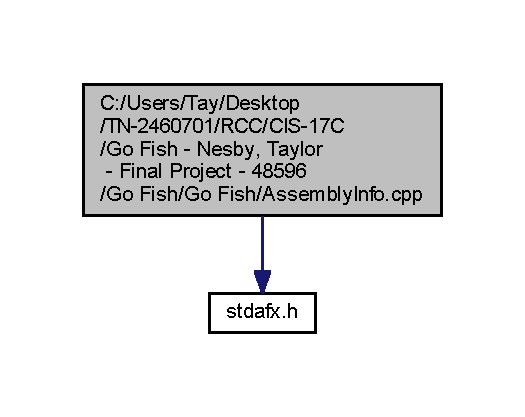
\includegraphics[width=252pt]{_assembly_info_8cpp__incl}
\end{center}
\end{figure}

\hypertarget{card_8h}{\section{C\+:/\+Users/\+Tay/\+Desktop/\+T\+N-\/2460701/\+R\+C\+C/\+C\+I\+S-\/17\+C/\+Go Fish -\/ Nesby, Taylor -\/ Final Project -\/ 48596/\+Go Fish/\+Go Fish/card.h File Reference}
\label{card_8h}\index{C\+:/\+Users/\+Tay/\+Desktop/\+T\+N-\/2460701/\+R\+C\+C/\+C\+I\+S-\/17\+C/\+Go Fish -\/ Nesby, Taylor -\/ Final Project -\/ 48596/\+Go Fish/\+Go Fish/card.\+h@{C\+:/\+Users/\+Tay/\+Desktop/\+T\+N-\/2460701/\+R\+C\+C/\+C\+I\+S-\/17\+C/\+Go Fish -\/ Nesby, Taylor -\/ Final Project -\/ 48596/\+Go Fish/\+Go Fish/card.\+h}}
}
This graph shows which files directly or indirectly include this file\+:\nopagebreak
\begin{figure}[H]
\begin{center}
\leavevmode
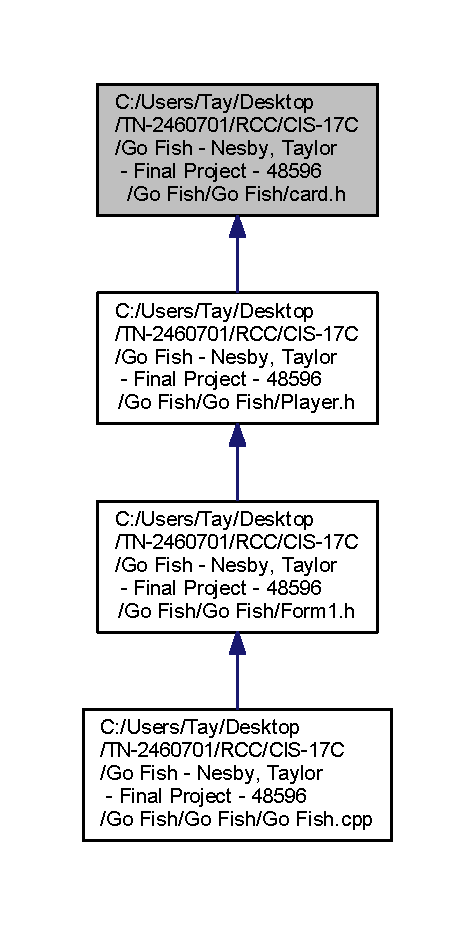
\includegraphics[width=228pt]{card_8h__dep__incl}
\end{center}
\end{figure}
\subsection*{Classes}
\begin{DoxyCompactItemize}
\item 
class \hyperlink{classcard}{card}
\end{DoxyCompactItemize}

\hypertarget{_form1_8h}{\section{C\+:/\+Users/\+Tay/\+Desktop/\+T\+N-\/2460701/\+R\+C\+C/\+C\+I\+S-\/17\+C/\+Go Fish -\/ Nesby, Taylor -\/ Final Project -\/ 48596/\+Go Fish/\+Go Fish/\+Form1.h File Reference}
\label{_form1_8h}\index{C\+:/\+Users/\+Tay/\+Desktop/\+T\+N-\/2460701/\+R\+C\+C/\+C\+I\+S-\/17\+C/\+Go Fish -\/ Nesby, Taylor -\/ Final Project -\/ 48596/\+Go Fish/\+Go Fish/\+Form1.\+h@{C\+:/\+Users/\+Tay/\+Desktop/\+T\+N-\/2460701/\+R\+C\+C/\+C\+I\+S-\/17\+C/\+Go Fish -\/ Nesby, Taylor -\/ Final Project -\/ 48596/\+Go Fish/\+Go Fish/\+Form1.\+h}}
}
{\ttfamily \#include $<$algorithm$>$}\\*
{\ttfamily \#include $<$cstdlib$>$}\\*
{\ttfamily \#include $<$map$>$}\\*
{\ttfamily \#include $<$sstream$>$}\\*
{\ttfamily \#include $<$ctime$>$}\\*
{\ttfamily \#include $<$string$>$}\\*
{\ttfamily \#include \char`\"{}Player.\+h\char`\"{}}\\*
{\ttfamily \#include \char`\"{}Tree.\+h\char`\"{}}\\*
Include dependency graph for Form1.\+h\+:\nopagebreak
\begin{figure}[H]
\begin{center}
\leavevmode
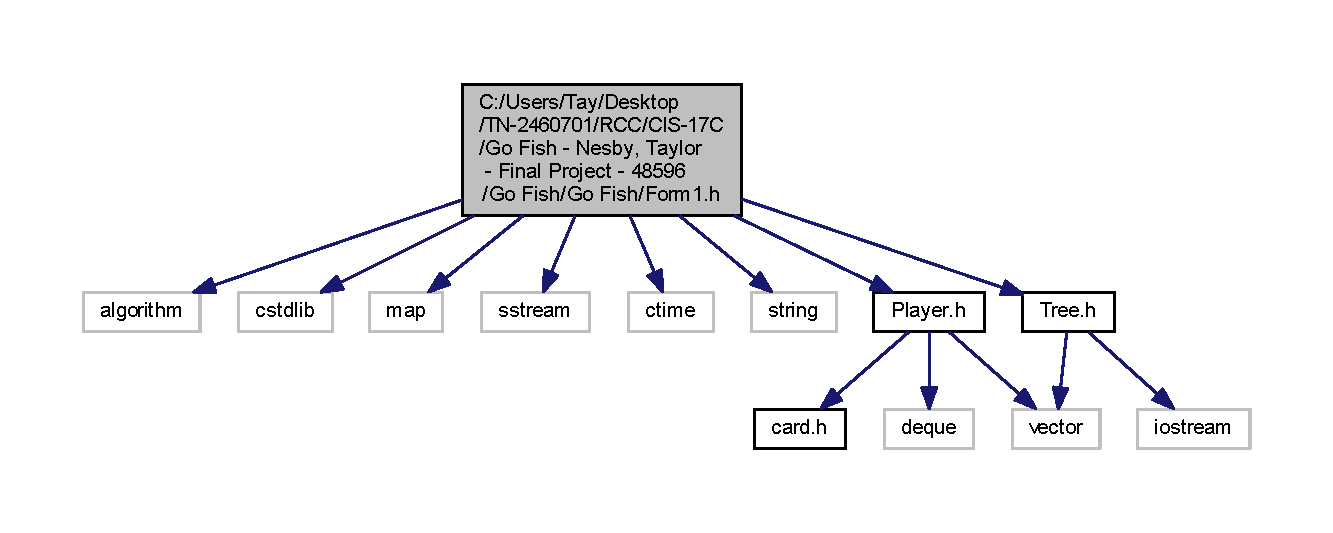
\includegraphics[width=350pt]{_form1_8h__incl}
\end{center}
\end{figure}
This graph shows which files directly or indirectly include this file\+:\nopagebreak
\begin{figure}[H]
\begin{center}
\leavevmode
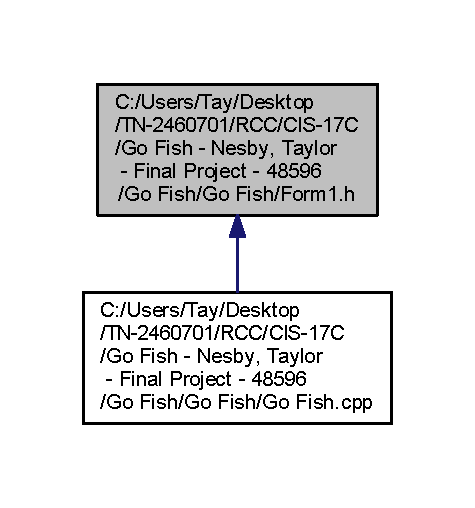
\includegraphics[width=228pt]{_form1_8h__dep__incl}
\end{center}
\end{figure}
\subsection*{Classes}
\begin{DoxyCompactItemize}
\item 
class \hyperlink{class_go_fish_1_1_form1}{Go\+Fish\+::\+Form1}
\end{DoxyCompactItemize}
\subsection*{Namespaces}
\begin{DoxyCompactItemize}
\item 
 \hyperlink{namespace_go_fish}{Go\+Fish}
\end{DoxyCompactItemize}
\subsection*{Functions}
\begin{DoxyCompactItemize}
\item 
map$<$ string, int $>$ \hyperlink{_form1_8h_a41e38e4a4b8b6d1e6ed17f2c44a158a3}{make\+Deck} ()
\item 
void \hyperlink{_form1_8h_aa395b22629e49d1ac5fa5a428dd443d1}{computer\+Action} ()
\item 
void \hyperlink{_form1_8h_af1136cb0c690066404d455bed14564d1}{update\+Hand} ()
\item 
void \hyperlink{_form1_8h_a51ae6a9f51032bbb696c44555f4fcf44}{update\+Score} ()
\item 
bool \hyperlink{_form1_8h_a73793f995211d82cca341e615d320c9f}{find\+Set} (\hyperlink{class_player}{Player} \&, int)
\item 
bool \hyperlink{_form1_8h_a23259daea96b5afbc49286e333e618b4}{winner} ()
\item 
void \hyperlink{_form1_8h_af60ac880dcd9513715ec22cbc66ea4f8}{remove\+Cards} (\hyperlink{class_player}{Player} \&x, int v, string g)
\end{DoxyCompactItemize}
\subsection*{Variables}
\begin{DoxyCompactItemize}
\item 
vector$<$ int $>$ \hyperlink{namespace_go_fish_a0516ae63daeafe7d734fd0e380a5cd24}{Go\+Fish\+::set}
\item 
deque$<$ \hyperlink{classcard}{card} $>$ \hyperlink{namespace_go_fish_aac69982a27bedb89f2ec4a108be9e7c1}{Go\+Fish\+::pool}
\item 
\hyperlink{class_player}{Player} \hyperlink{namespace_go_fish_a9fdd5a69166f90eee7f9717e376ea9bb}{Go\+Fish\+::computer}
\item 
\hyperlink{class_player}{Player} \hyperlink{namespace_go_fish_ad4928743b77010f80388ae5f5495bb1b}{Go\+Fish\+::person}
\item 
bool \hyperlink{namespace_go_fish_a5ef343351958e4a4c45cfa2d0aa895b5}{Go\+Fish\+::wrong} =true
\item 
bool \hyperlink{namespace_go_fish_a76b216755d7556d9ee96ca7ae0fa620d}{Go\+Fish\+::time\+To\+Draw} =false
\item 
bool \hyperlink{namespace_go_fish_a1e5e3f29ab64f86a067ee143e1ca2996}{Go\+Fish\+::computer\+Turn} =false
\item 
bool \hyperlink{namespace_go_fish_af285f106abe3d068160690d582c4ec70}{Go\+Fish\+::time\+To\+Submit} =false
\item 
int \hyperlink{namespace_go_fish_a678c54ee6f4ee2d5eb6ddc8922c1f38d}{Go\+Fish\+::person\+Count} =0
\item 
int \hyperlink{namespace_go_fish_a9e05ca6eb20a4dbd5eedd1ed0540de91}{Go\+Fish\+::computer\+Count} =0
\end{DoxyCompactItemize}


\subsection{Function Documentation}
\hypertarget{_form1_8h_aa395b22629e49d1ac5fa5a428dd443d1}{\index{Form1.\+h@{Form1.\+h}!computer\+Action@{computer\+Action}}
\index{computer\+Action@{computer\+Action}!Form1.\+h@{Form1.\+h}}
\subsubsection[{computer\+Action}]{\setlength{\rightskip}{0pt plus 5cm}void computer\+Action (
\begin{DoxyParamCaption}
{}
\end{DoxyParamCaption}
)}}\label{_form1_8h_aa395b22629e49d1ac5fa5a428dd443d1}
\hypertarget{_form1_8h_a73793f995211d82cca341e615d320c9f}{\index{Form1.\+h@{Form1.\+h}!find\+Set@{find\+Set}}
\index{find\+Set@{find\+Set}!Form1.\+h@{Form1.\+h}}
\subsubsection[{find\+Set}]{\setlength{\rightskip}{0pt plus 5cm}bool find\+Set (
\begin{DoxyParamCaption}
\item[{{\bf Player} \&}]{, }
\item[{int}]{}
\end{DoxyParamCaption}
)}}\label{_form1_8h_a73793f995211d82cca341e615d320c9f}


Here is the caller graph for this function\+:\nopagebreak
\begin{figure}[H]
\begin{center}
\leavevmode
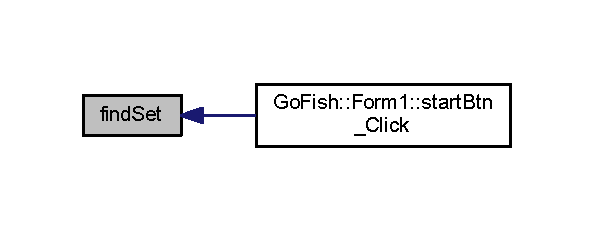
\includegraphics[width=285pt]{_form1_8h_a73793f995211d82cca341e615d320c9f_icgraph}
\end{center}
\end{figure}


\hypertarget{_form1_8h_a41e38e4a4b8b6d1e6ed17f2c44a158a3}{\index{Form1.\+h@{Form1.\+h}!make\+Deck@{make\+Deck}}
\index{make\+Deck@{make\+Deck}!Form1.\+h@{Form1.\+h}}
\subsubsection[{make\+Deck}]{\setlength{\rightskip}{0pt plus 5cm}map$<$ string, int $>$ make\+Deck (
\begin{DoxyParamCaption}
{}
\end{DoxyParamCaption}
)}}\label{_form1_8h_a41e38e4a4b8b6d1e6ed17f2c44a158a3}


Definition at line 959 of file Form1.\+h.



Here is the caller graph for this function\+:\nopagebreak
\begin{figure}[H]
\begin{center}
\leavevmode
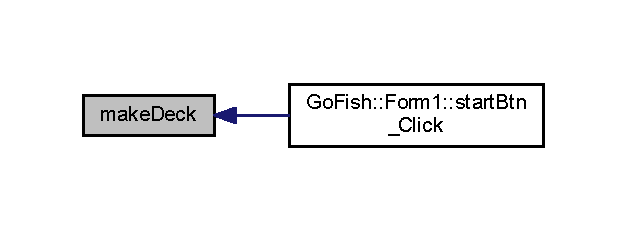
\includegraphics[width=301pt]{_form1_8h_a41e38e4a4b8b6d1e6ed17f2c44a158a3_icgraph}
\end{center}
\end{figure}


\hypertarget{_form1_8h_af60ac880dcd9513715ec22cbc66ea4f8}{\index{Form1.\+h@{Form1.\+h}!remove\+Cards@{remove\+Cards}}
\index{remove\+Cards@{remove\+Cards}!Form1.\+h@{Form1.\+h}}
\subsubsection[{remove\+Cards}]{\setlength{\rightskip}{0pt plus 5cm}void remove\+Cards (
\begin{DoxyParamCaption}
\item[{{\bf Player} \&}]{x, }
\item[{int}]{v, }
\item[{string}]{g}
\end{DoxyParamCaption}
)}}\label{_form1_8h_af60ac880dcd9513715ec22cbc66ea4f8}


Definition at line 1016 of file Form1.\+h.

\hypertarget{_form1_8h_af1136cb0c690066404d455bed14564d1}{\index{Form1.\+h@{Form1.\+h}!update\+Hand@{update\+Hand}}
\index{update\+Hand@{update\+Hand}!Form1.\+h@{Form1.\+h}}
\subsubsection[{update\+Hand}]{\setlength{\rightskip}{0pt plus 5cm}void update\+Hand (
\begin{DoxyParamCaption}
{}
\end{DoxyParamCaption}
)}}\label{_form1_8h_af1136cb0c690066404d455bed14564d1}


Here is the caller graph for this function\+:\nopagebreak
\begin{figure}[H]
\begin{center}
\leavevmode
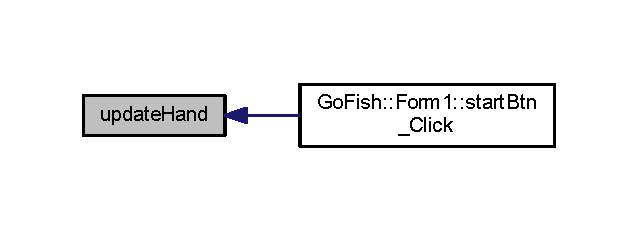
\includegraphics[width=306pt]{_form1_8h_af1136cb0c690066404d455bed14564d1_icgraph}
\end{center}
\end{figure}


\hypertarget{_form1_8h_a51ae6a9f51032bbb696c44555f4fcf44}{\index{Form1.\+h@{Form1.\+h}!update\+Score@{update\+Score}}
\index{update\+Score@{update\+Score}!Form1.\+h@{Form1.\+h}}
\subsubsection[{update\+Score}]{\setlength{\rightskip}{0pt plus 5cm}void update\+Score (
\begin{DoxyParamCaption}
{}
\end{DoxyParamCaption}
)}}\label{_form1_8h_a51ae6a9f51032bbb696c44555f4fcf44}


Here is the caller graph for this function\+:\nopagebreak
\begin{figure}[H]
\begin{center}
\leavevmode
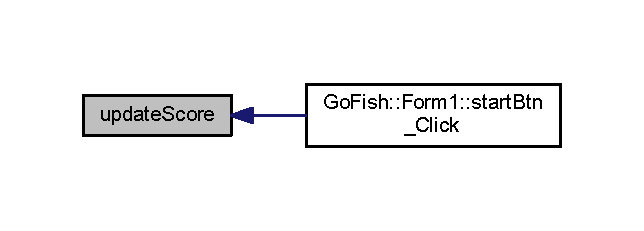
\includegraphics[width=309pt]{_form1_8h_a51ae6a9f51032bbb696c44555f4fcf44_icgraph}
\end{center}
\end{figure}


\hypertarget{_form1_8h_a23259daea96b5afbc49286e333e618b4}{\index{Form1.\+h@{Form1.\+h}!winner@{winner}}
\index{winner@{winner}!Form1.\+h@{Form1.\+h}}
\subsubsection[{winner}]{\setlength{\rightskip}{0pt plus 5cm}bool winner (
\begin{DoxyParamCaption}
{}
\end{DoxyParamCaption}
)}}\label{_form1_8h_a23259daea96b5afbc49286e333e618b4}

\hypertarget{_go_01_fish_8cpp}{\section{C\+:/\+Users/\+Tay/\+Desktop/\+T\+N-\/2460701/\+R\+C\+C/\+C\+I\+S-\/17\+C/\+Go Fish -\/ Nesby, Taylor -\/ Final Project -\/ 48596/\+Go Fish/\+Go Fish/\+Go Fish.\+cpp File Reference}
\label{_go_01_fish_8cpp}\index{C\+:/\+Users/\+Tay/\+Desktop/\+T\+N-\/2460701/\+R\+C\+C/\+C\+I\+S-\/17\+C/\+Go Fish -\/ Nesby, Taylor -\/ Final Project -\/ 48596/\+Go Fish/\+Go Fish/\+Go Fish.\+cpp@{C\+:/\+Users/\+Tay/\+Desktop/\+T\+N-\/2460701/\+R\+C\+C/\+C\+I\+S-\/17\+C/\+Go Fish -\/ Nesby, Taylor -\/ Final Project -\/ 48596/\+Go Fish/\+Go Fish/\+Go Fish.\+cpp}}
}
{\ttfamily \#include \char`\"{}stdafx.\+h\char`\"{}}\\*
{\ttfamily \#include \char`\"{}Form1.\+h\char`\"{}}\\*
Include dependency graph for Go Fish.\+cpp\+:\nopagebreak
\begin{figure}[H]
\begin{center}
\leavevmode
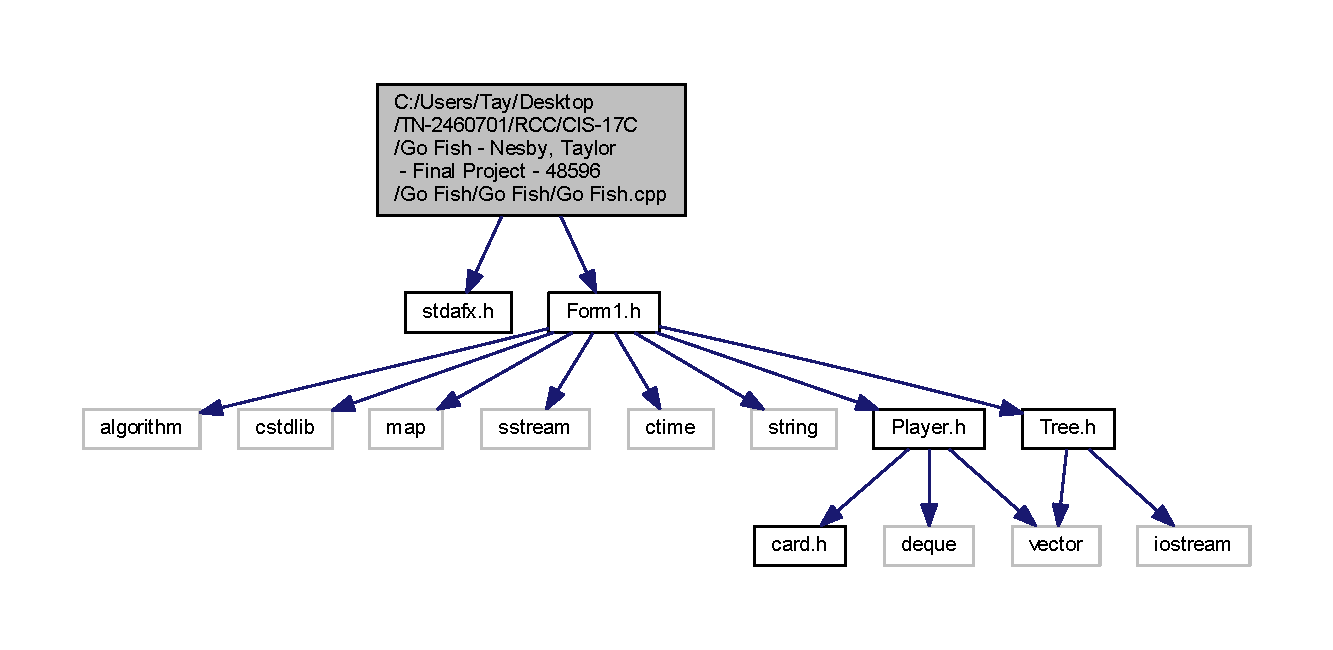
\includegraphics[width=350pt]{_go_01_fish_8cpp__incl}
\end{center}
\end{figure}
\subsection*{Functions}
\begin{DoxyCompactItemize}
\item 
int \hyperlink{_go_01_fish_8cpp_ac7eb149011d4000560640a5ad21683fe}{main} (array$<$ System\+::\+String$^\wedge$$>$$^\wedge$args)
\end{DoxyCompactItemize}


\subsection{Function Documentation}
\hypertarget{_go_01_fish_8cpp_ac7eb149011d4000560640a5ad21683fe}{\index{Go Fish.\+cpp@{Go Fish.\+cpp}!main@{main}}
\index{main@{main}!Go Fish.\+cpp@{Go Fish.\+cpp}}
\subsubsection[{main}]{\setlength{\rightskip}{0pt plus 5cm}int main (
\begin{DoxyParamCaption}
\item[{array$<$ System\+::\+String$^\wedge$$>$$^\wedge$}]{args}
\end{DoxyParamCaption}
)}}\label{_go_01_fish_8cpp_ac7eb149011d4000560640a5ad21683fe}


Definition at line 9 of file Go Fish.\+cpp.


\hypertarget{_player_8h}{\section{C\+:/\+Users/\+Tay/\+Desktop/\+T\+N-\/2460701/\+R\+C\+C/\+C\+I\+S-\/17\+C/\+Go Fish -\/ Nesby, Taylor -\/ Final Project -\/ 48596/\+Go Fish/\+Go Fish/\+Player.h File Reference}
\label{_player_8h}\index{C\+:/\+Users/\+Tay/\+Desktop/\+T\+N-\/2460701/\+R\+C\+C/\+C\+I\+S-\/17\+C/\+Go Fish -\/ Nesby, Taylor -\/ Final Project -\/ 48596/\+Go Fish/\+Go Fish/\+Player.\+h@{C\+:/\+Users/\+Tay/\+Desktop/\+T\+N-\/2460701/\+R\+C\+C/\+C\+I\+S-\/17\+C/\+Go Fish -\/ Nesby, Taylor -\/ Final Project -\/ 48596/\+Go Fish/\+Go Fish/\+Player.\+h}}
}
{\ttfamily \#include \char`\"{}card.\+h\char`\"{}}\\*
{\ttfamily \#include $<$vector$>$}\\*
{\ttfamily \#include $<$deque$>$}\\*
Include dependency graph for Player.\+h\+:\nopagebreak
\begin{figure}[H]
\begin{center}
\leavevmode
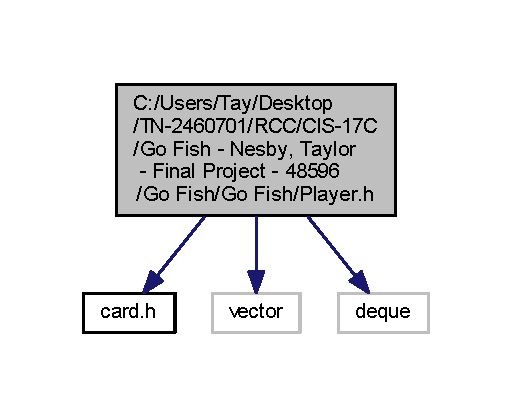
\includegraphics[width=246pt]{_player_8h__incl}
\end{center}
\end{figure}
This graph shows which files directly or indirectly include this file\+:\nopagebreak
\begin{figure}[H]
\begin{center}
\leavevmode
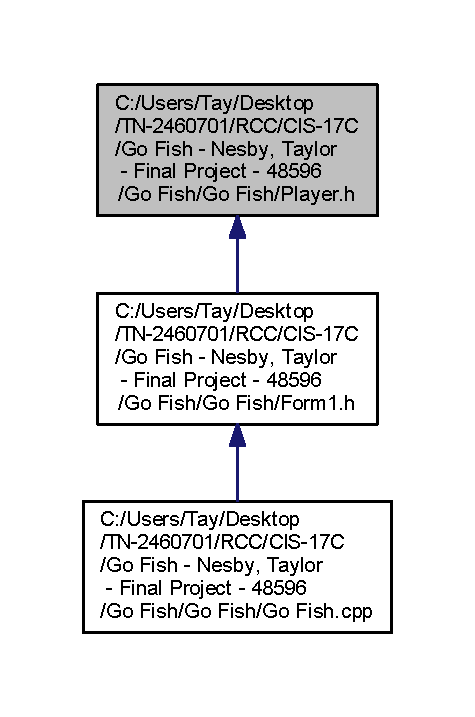
\includegraphics[width=228pt]{_player_8h__dep__incl}
\end{center}
\end{figure}
\subsection*{Classes}
\begin{DoxyCompactItemize}
\item 
class \hyperlink{class_player}{Player}
\end{DoxyCompactItemize}

\hypertarget{resource_8h}{\section{C\+:/\+Users/\+Tay/\+Desktop/\+T\+N-\/2460701/\+R\+C\+C/\+C\+I\+S-\/17\+C/\+Go Fish -\/ Nesby, Taylor -\/ Final Project -\/ 48596/\+Go Fish/\+Go Fish/resource.h File Reference}
\label{resource_8h}\index{C\+:/\+Users/\+Tay/\+Desktop/\+T\+N-\/2460701/\+R\+C\+C/\+C\+I\+S-\/17\+C/\+Go Fish -\/ Nesby, Taylor -\/ Final Project -\/ 48596/\+Go Fish/\+Go Fish/resource.\+h@{C\+:/\+Users/\+Tay/\+Desktop/\+T\+N-\/2460701/\+R\+C\+C/\+C\+I\+S-\/17\+C/\+Go Fish -\/ Nesby, Taylor -\/ Final Project -\/ 48596/\+Go Fish/\+Go Fish/resource.\+h}}
}

\hypertarget{stdafx_8cpp}{\section{C\+:/\+Users/\+Tay/\+Desktop/\+T\+N-\/2460701/\+R\+C\+C/\+C\+I\+S-\/17\+C/\+Go Fish -\/ Nesby, Taylor -\/ Final Project -\/ 48596/\+Go Fish/\+Go Fish/stdafx.cpp File Reference}
\label{stdafx_8cpp}\index{C\+:/\+Users/\+Tay/\+Desktop/\+T\+N-\/2460701/\+R\+C\+C/\+C\+I\+S-\/17\+C/\+Go Fish -\/ Nesby, Taylor -\/ Final Project -\/ 48596/\+Go Fish/\+Go Fish/stdafx.\+cpp@{C\+:/\+Users/\+Tay/\+Desktop/\+T\+N-\/2460701/\+R\+C\+C/\+C\+I\+S-\/17\+C/\+Go Fish -\/ Nesby, Taylor -\/ Final Project -\/ 48596/\+Go Fish/\+Go Fish/stdafx.\+cpp}}
}
{\ttfamily \#include \char`\"{}stdafx.\+h\char`\"{}}\\*
Include dependency graph for stdafx.\+cpp\+:\nopagebreak
\begin{figure}[H]
\begin{center}
\leavevmode
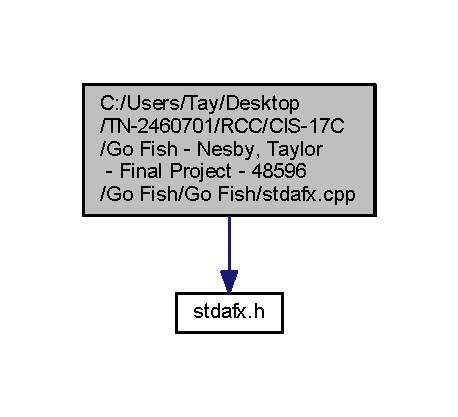
\includegraphics[width=220pt]{stdafx_8cpp__incl}
\end{center}
\end{figure}

\hypertarget{stdafx_8h}{\section{C\+:/\+Users/\+Tay/\+Desktop/\+T\+N-\/2460701/\+R\+C\+C/\+C\+I\+S-\/17\+C/\+Go Fish -\/ Nesby, Taylor -\/ Final Project -\/ 48596/\+Go Fish/\+Go Fish/stdafx.h File Reference}
\label{stdafx_8h}\index{C\+:/\+Users/\+Tay/\+Desktop/\+T\+N-\/2460701/\+R\+C\+C/\+C\+I\+S-\/17\+C/\+Go Fish -\/ Nesby, Taylor -\/ Final Project -\/ 48596/\+Go Fish/\+Go Fish/stdafx.\+h@{C\+:/\+Users/\+Tay/\+Desktop/\+T\+N-\/2460701/\+R\+C\+C/\+C\+I\+S-\/17\+C/\+Go Fish -\/ Nesby, Taylor -\/ Final Project -\/ 48596/\+Go Fish/\+Go Fish/stdafx.\+h}}
}
This graph shows which files directly or indirectly include this file\+:\nopagebreak
\begin{figure}[H]
\begin{center}
\leavevmode
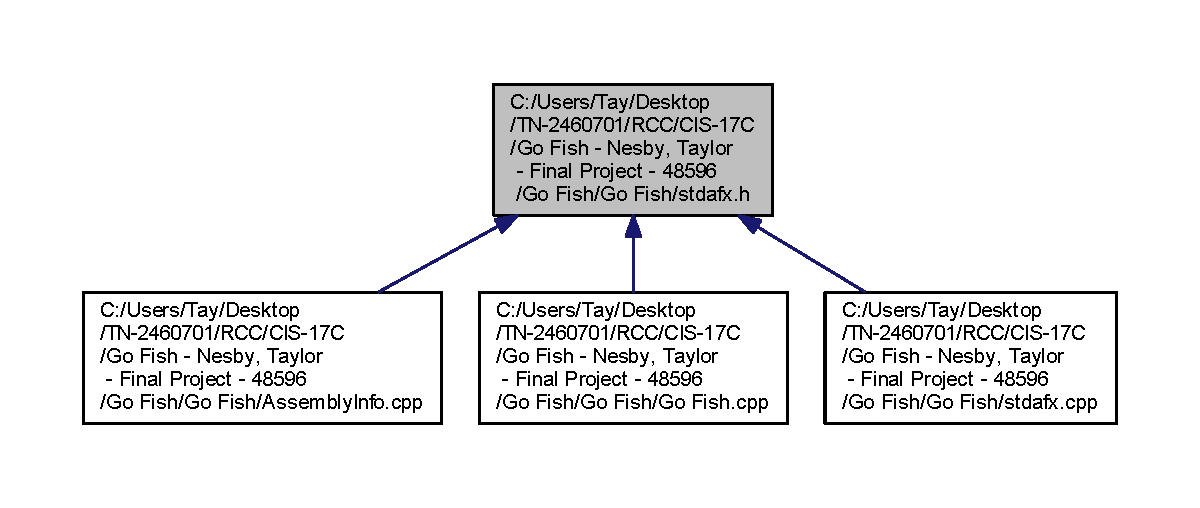
\includegraphics[width=350pt]{stdafx_8h__dep__incl}
\end{center}
\end{figure}

\hypertarget{_tree_8h}{\section{C\+:/\+Users/\+Tay/\+Desktop/\+T\+N-\/2460701/\+R\+C\+C/\+C\+I\+S-\/17\+C/\+Go Fish -\/ Nesby, Taylor -\/ Final Project -\/ 48596/\+Go Fish/\+Go Fish/\+Tree.h File Reference}
\label{_tree_8h}\index{C\+:/\+Users/\+Tay/\+Desktop/\+T\+N-\/2460701/\+R\+C\+C/\+C\+I\+S-\/17\+C/\+Go Fish -\/ Nesby, Taylor -\/ Final Project -\/ 48596/\+Go Fish/\+Go Fish/\+Tree.\+h@{C\+:/\+Users/\+Tay/\+Desktop/\+T\+N-\/2460701/\+R\+C\+C/\+C\+I\+S-\/17\+C/\+Go Fish -\/ Nesby, Taylor -\/ Final Project -\/ 48596/\+Go Fish/\+Go Fish/\+Tree.\+h}}
}
{\ttfamily \#include $<$iostream$>$}\\*
{\ttfamily \#include $<$vector$>$}\\*
Include dependency graph for Tree.\+h\+:\nopagebreak
\begin{figure}[H]
\begin{center}
\leavevmode
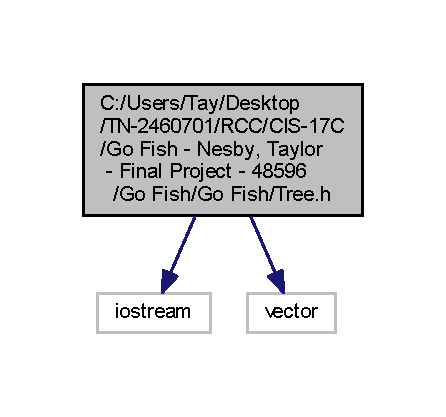
\includegraphics[width=214pt]{_tree_8h__incl}
\end{center}
\end{figure}
This graph shows which files directly or indirectly include this file\+:\nopagebreak
\begin{figure}[H]
\begin{center}
\leavevmode
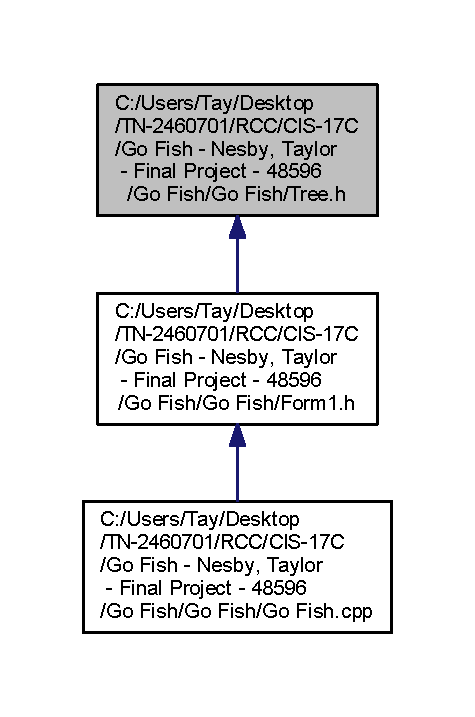
\includegraphics[width=228pt]{_tree_8h__dep__incl}
\end{center}
\end{figure}
\subsection*{Classes}
\begin{DoxyCompactItemize}
\item 
class \hyperlink{class_tree}{Tree}
\end{DoxyCompactItemize}

%--- End generated contents ---

% Index
\newpage
\phantomsection
\addcontentsline{toc}{chapter}{Index}
\printindex

\end{document}
